% Numeric oracle for TikZ's fixed-point to-path distance and shape clipping.
\documentclass{article}
\usepackage{tikz}
\usetikzlibrary{arrows,shapes.geometric,bending}
\begin{document}
\makeatletter
\newcommand{\reportdistance}[2]{%
  \def\tikz@first@point{\pgfpoint{0pt}{0pt}}%
  \def\tikz@second@point{\pgfpoint{#1}{#2}}%
  \tikz@to@compute@distance@main
  \typeout{DISTANCE (#1,#2): \the\pgf@xa,\the\pgf@xb}}
\newcommand{\reportpath}[1]{%
  \pgfgetpath\savedpath
  \typeout{PATH #1: \meaning\savedpath}}
\reportdistance{4cm}{0cm}
\reportdistance{2cm}{0cm}
\reportdistance{0cm}{4cm}
\reportdistance{3cm}{4cm}
\reportdistance{4cm}{3cm}
\reportdistance{1cm}{1cm}
\reportdistance{4cm}{0.001pt}
\reportdistance{0cm}{0cm}
\reportdistance{0.01pt}{0.02pt}
\foreach \angle in {0,.5,...,90}{%
  \pgfpointpolar{\angle}{4cm}
  \edef\xx{\the\pgf@x}\edef\yy{\the\pgf@y}
  \reportdistance{\xx}{\yy}}
\begin{tikzpicture}
  \draw (0,0) to[out=20,in=160] (4,0) \pgfextra{%
    \reportpath{bare}
    % The native control points are reported immediately above.
    \pgfsetcurvilinearbeziercurve{\pgfpoint{113.81097pt}{0pt}}{\pgfpoint{72.10446pt}{15.1801pt}}{\pgfpoint{41.70651pt}{15.1801pt}}{\pgfpoint{0pt}{0pt}}
    \typeout{CURVE TABLE: \the\pgf@curvilinear@time@a;\the\pgf@curvilinear@length@a;\the\pgf@curvilinear@length@b;\the\pgf@curvilinear@length@c;\the\pgf@curvilinear@length@d}
    \foreach \distance in {-1pt,1pt,3pt,6.6pt,10pt}{%
      \pgfcurvilineardistancetotime{\distance}
      \typeout{CURVE TIME \distance: \the\pgf@x}
      \typeout{CURVE QUOT: \meaning\pgf@curvilinear@quot@d;\meaning\pgf@curvilinear@correct@d}}
    \pgfsetcurvilinearbeziercurve{\pgfpoint{113.81097pt}{0pt}}{\pgfpoint{72.10446pt}{15.1801pt}}{\pgfpoint{41.70651pt}{15.1801pt}}{\pgfpoint{0pt}{0pt}}
    \typeout{CURVE REPEATED TABLE: \the\pgf@curvilinear@time@a;\the\pgf@curvilinear@length@a}};
  \node[draw,minimum width=.5cm,minimum height=.3cm] (a) at (0,0) {A};
  \node[draw,minimum width=.5cm,minimum height=.3cm] (b) at (2,0) {B};
  \draw (a) to[out=20,in=160] (b) \pgfextra{\reportpath{plain}};
  \draw[-stealth] (a) to[out=20,in=160] (b) \pgfextra{\reportpath{arrow}};
  \draw[<->,line width=4pt] (a) to[out=20,in=160] (b) \pgfextra{\reportpath{thick}};
  \draw[-stealth] (a.20) to[out=20,in=160] (b.160) \pgfextra{\reportpath{anchors}};
  \node[draw,circle,minimum size=1cm,inner sep=0pt] (c) at (0,-2) {};
  \node[draw,ellipse,minimum width=2cm,minimum height=1cm,inner sep=0pt] (d) at (4,-2) {};
  \draw[line width=4pt,-stealth] (c) to[out=25,in=145] (d) \pgfextra{\reportpath{circle-ellipse}};
\end{tikzpicture}
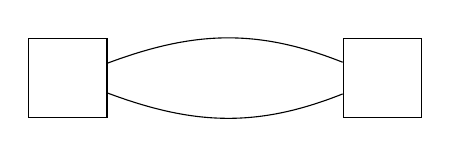
\begin{tikzpicture}
  \node[draw,minimum size=1cm,inner sep=0pt] (a) at (0,0) {};
  \node[draw,minimum size=1cm,inner sep=0pt] (b) at (4,0) {};
  \draw (a) to[out=20.75,in=158.5] (b) \pgfextra{\reportpath{fractional-positive}};
  \draw (a) to[out=-20.75,in=-158.5] (b) \pgfextra{\reportpath{fractional-negative}};
\end{tikzpicture}
\makeatother
\end{document}
